\documentclass{tufte-handout}

\title{Ultimate frisbee: strategy and tactics: O1}
\author[James Reynolds]{James Reynolds}

%\date{28 March 2010} % without \date command, current date is supplied

%\geometry{showframe} % display margins for debugging page layout

\usepackage{graphicx} % allow embedded images
  \setkeys{Gin}{width=\linewidth,totalheight=\textheight,keepaspectratio}
  \graphicspath{{graphics/}} % set of paths to search for images
\usepackage{amsmath}  % extended mathematics
\usepackage{booktabs} % book-quality tables
\usepackage{units}    % non-stacked fractions and better unit spacing
\usepackage{multicol} % multiple column layout facilities
\usepackage{lipsum}   % filler text
\usepackage{fancyvrb} % extended verbatim environments
  \fvset{fontsize=\normalsize}% default font size for fancy-verbatim environments

% Standardize command font styles and environments
\newcommand{\doccmd}[1]{\texttt{\textbackslash#1}}% command name -- adds backslash automatically
\newcommand{\docopt}[1]{\ensuremath{\langle}\textrm{\textit{#1}}\ensuremath{\rangle}}% optional command argument
\newcommand{\docarg}[1]{\textrm{\textit{#1}}}% (required) command argument
\newcommand{\docenv}[1]{\textsf{#1}}% environment name
\newcommand{\docpkg}[1]{\texttt{#1}}% package name
\newcommand{\doccls}[1]{\texttt{#1}}% document class name
\newcommand{\docclsopt}[1]{\texttt{#1}}% document class option name
\newenvironment{docspec}{\begin{quote}\noindent}{\end{quote}}% command specification environment

\begin{document}

\maketitle% this prints the handout title, author, and date


\begin{marginfigure}%
  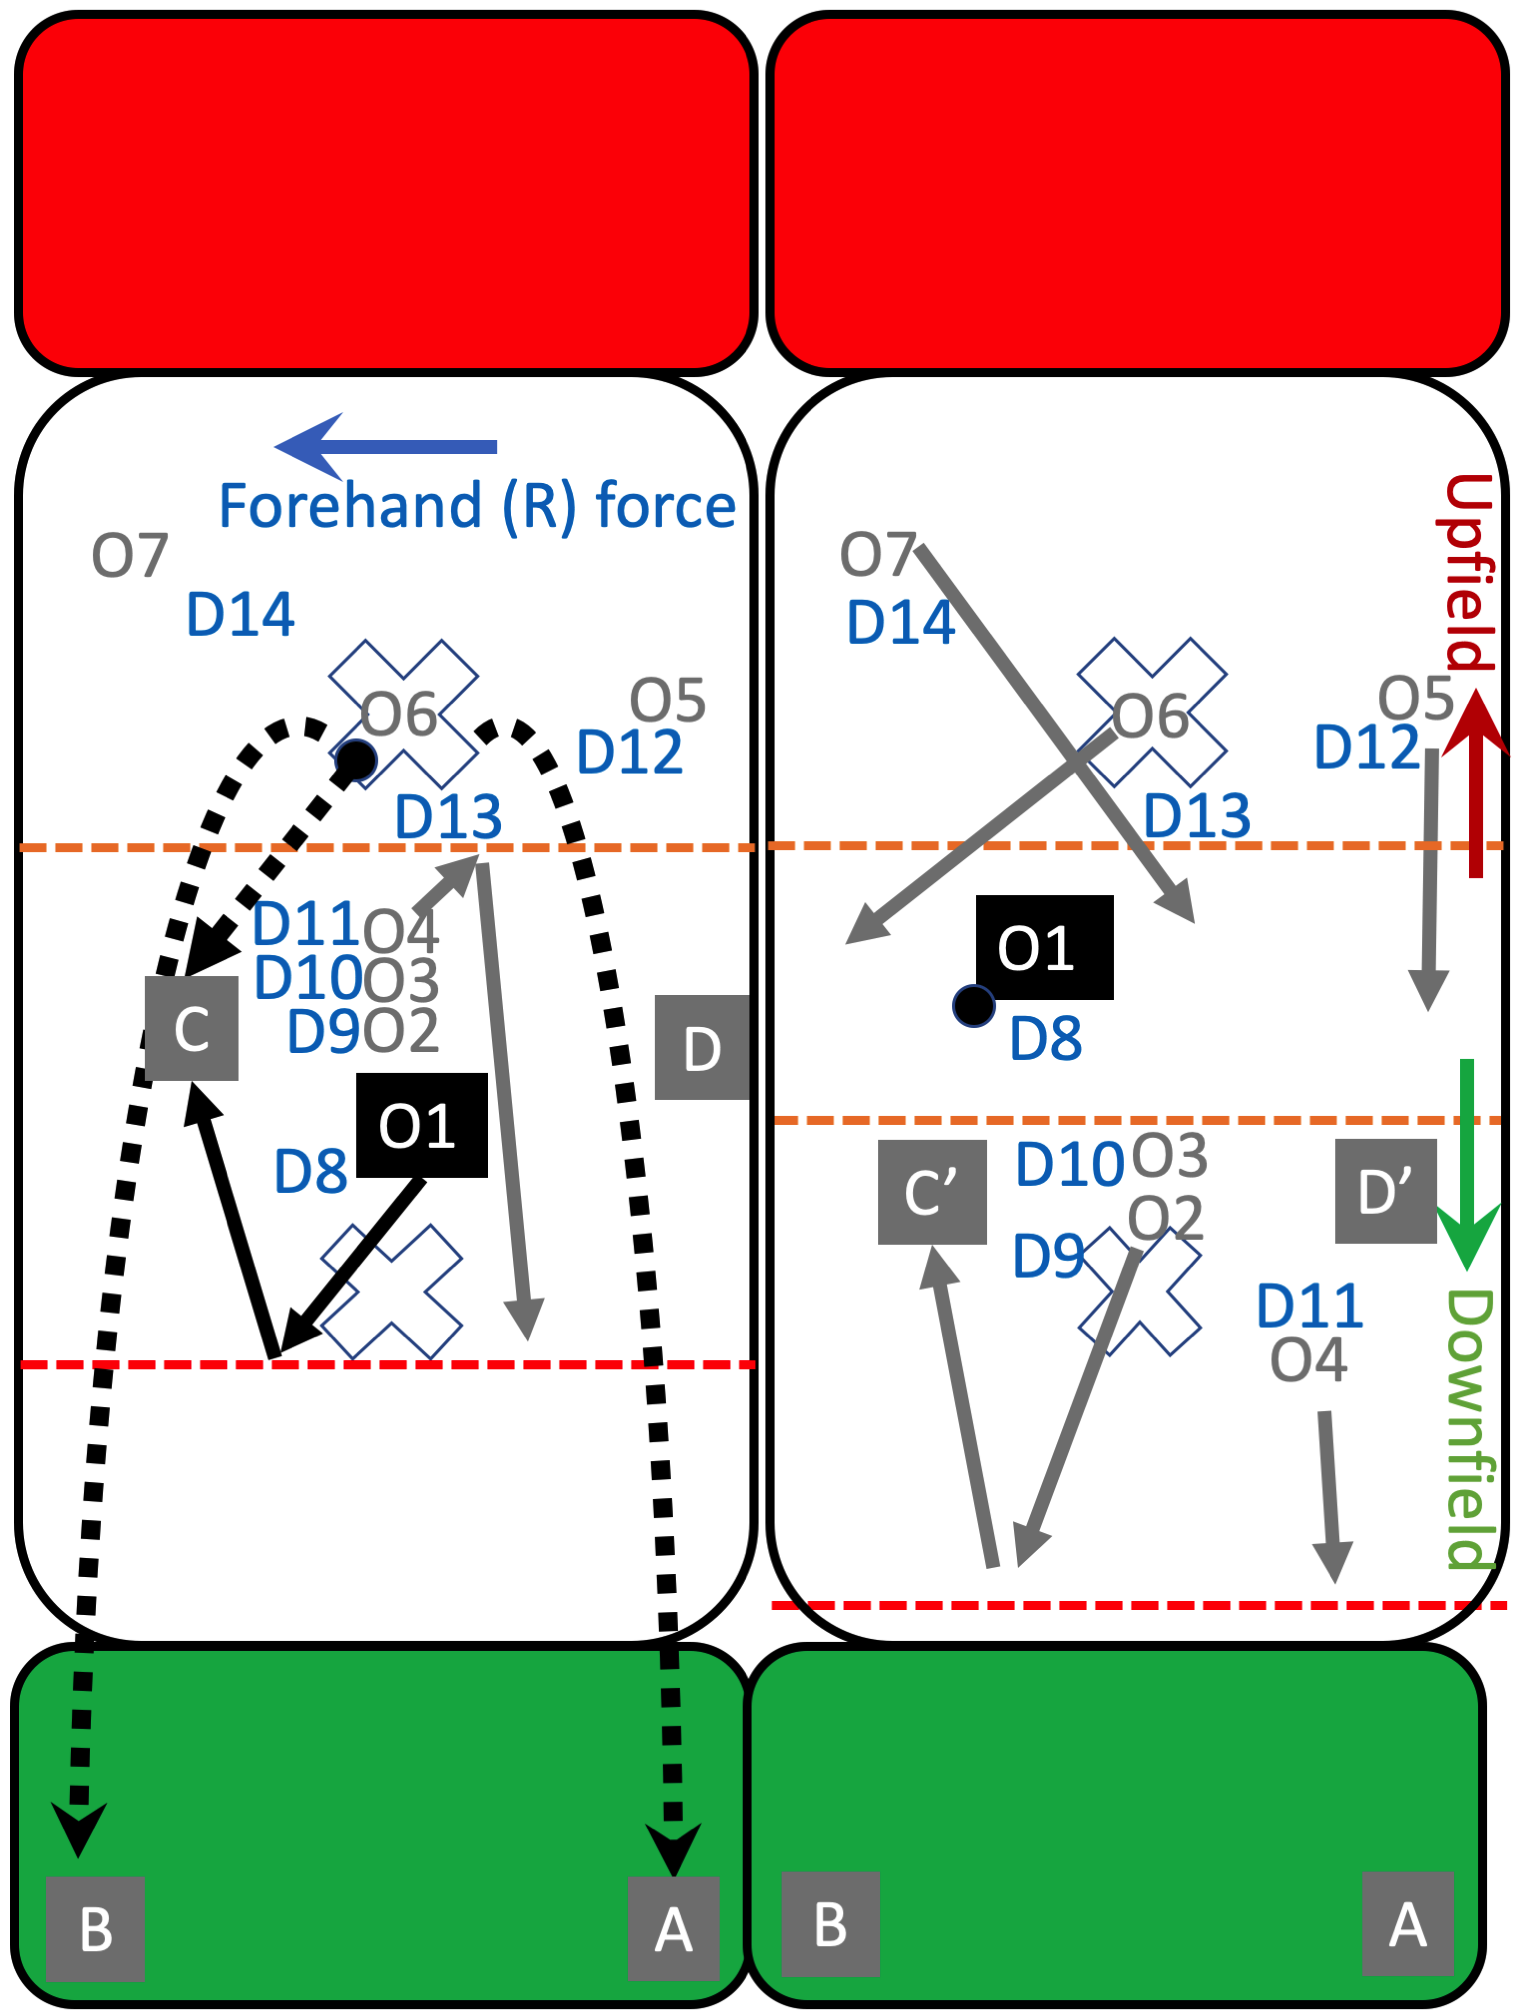
\includegraphics[width=\linewidth]{O1-vertical}
  \caption{Vertical stack formation}
  \label{fig:O1-vertical}
\end{marginfigure}



%\printclassoptions
This document is about 
playing primary 'middle' 
or left wing 
on offence,
referred to as position O1 here\footnote{This
is part of a series, 
available here (LINK TO BE PROVIDED}.
\newthought{Your team is starting the point} on offence. 
After the pull 
as you run downfield\footnote{
In the meantime, 
the handlers on your team 
will be busy 
catching the pull
Figures \ref{fig:O1-vertical} and  \ref{fig:O1-horizontal} 
show O6 starting play 
at the brick mark, 
as might occur if 
the pull is out.} 
it will help 
if you can figure out 
what defensive structure the D team 
is using:
person-match defence;
a traditional 3-3-1 zone defence; or
something else\footnote{
person-match-last-back-helps,
person-match-with-a-poacher,
Person-match-with-lots-of switching,
force-middle,
Force-straight-up
3-2-2, 
2-3-2, 
1-3-2-1 (puppy-fence),
clam,
etc.}.

\section{Person-match defence, RH forehand force: vertical stack}\label{sec:vertical}
Figure \ref{fig:O1-vertical} shows 
O6 throwing you either:
\begin{enumerate}
\item a break-side 
huck to A\footnote{
This throw is 
probably
very difficult. 
However, you as O1
will just have to
stand still 
till O6 throws it, 
then run and catch it.
Figure \ref{fig:O1-vertical} indicates how 
D8 will be on the wrong side of you (as O1)
and so probably won't have much of a play on the disc.};
\item an open-side huck to B\footnote{
Especially viable if: 
D8 closer to the disc than (upfield of) you; 
you are faster than D8; or 
D8 does not react to an initial cut downfield (black arrow)}; or 
\item an open-side throw 
to an upfield cut to C\footnote{
The solid black arrows indicate 
a cut you might do;
initially going deep,
but then back-under
(upfield)
on the open side.}.
\end{enumerate}


It’s good to restrict your cutting 
to between 
the dashed red 
and dashed yellow lines. 
If you go 
downfield of the dashed red line 
before O6 throws the disc\footnote{
A, B 
and the dashed red line 
effectively move further upfield
or downfield
if O6 has a shorter or longer huck.},
D8 will be able 
get to
A or B 
before the disc,
intercepting 
or preventing 
deep throws to 
you or others. 
Similarly, 
You being 
upfield of the dashed yellow line
lets D8
prevent dump throws from O6
to O5 
or O7.
Hence,
if you cut to C
but the disc is not thrown to you
perhaps cut downfield again,
then return to the stack
and make space for other cutters. 

Figure \ref{fig:O1-vertical2} shows 
the disc having been thrown to you
on the back-under cut towards C \footnote{
Note that A', B', C', and 
the yellow and red dashed lines 
are all now further downfield 
reflecting the new position of the disc.
The stack (O2, O3) 
has also moved downfield.}.

\begin{marginfigure}%
  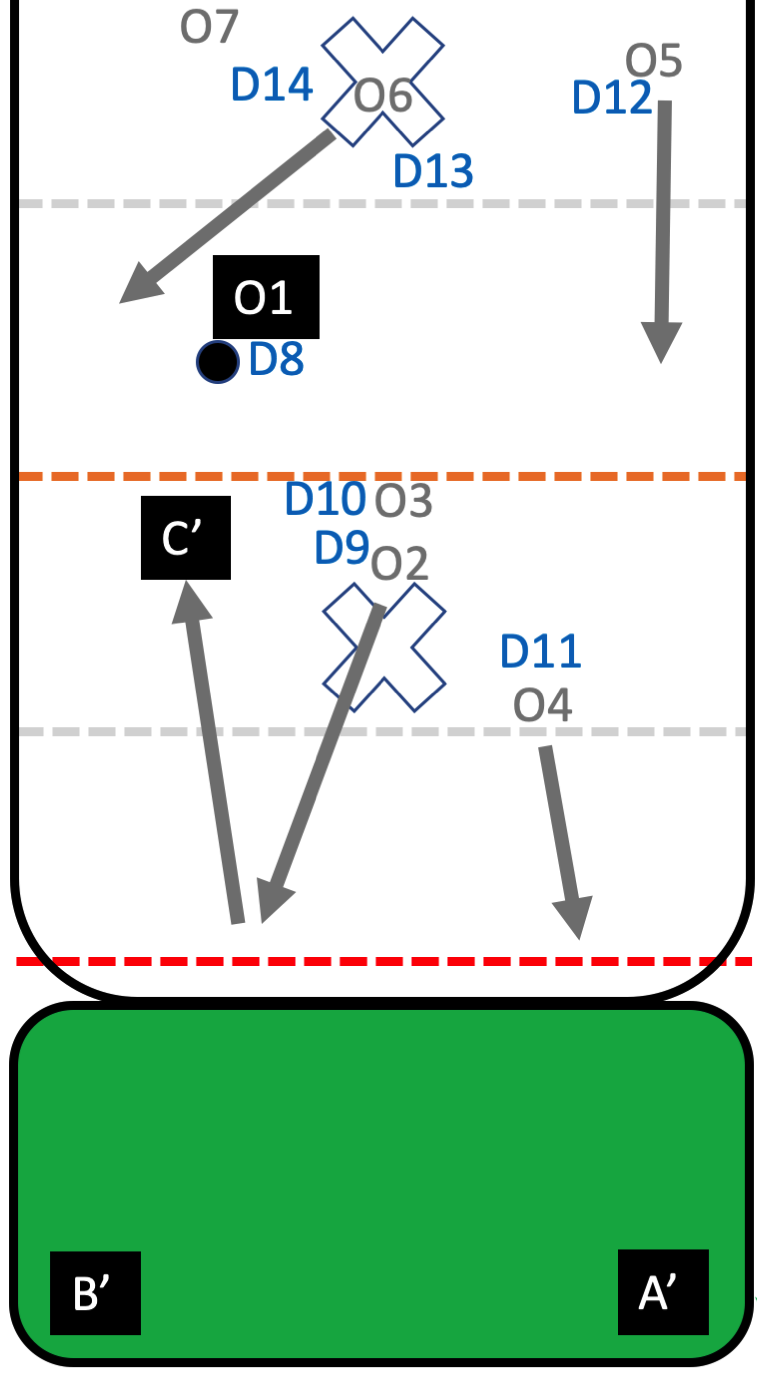
\includegraphics[width=\linewidth]{O1-vertical2}
  \caption{Vertical stack progression}
  \label{fig:O1-vertical2}
\end{marginfigure}

Your options include:
\begin{enumerate}
\item throwing to O2 or O4 at A'
(to O4 or maybe O2);
\item throwing to O2 at B' or C', 
using the same cutting approach
you did earlier;
\item off-load to O6 
moving downfield and right\footnote{
Grey arrow. 
A pass to O6 
should be relatively easy, 
as D13 is on the wrong side having been forcing O6 forehand earlier.   
This pass would put O6
in 'power poistion'
where they can easily 
thrown anywhere on the field 
as D13 will likely be behind them. 
In contrast, D8 
will be downfield 
of you
making it easier for them to 
apply the force.};
\item break the force 
to throw to O3 
or O5; or 
\item
throw a dump to O7.
\end{enumerate}
Next, get back to the stack
or make another cut.


\section{Person-match defence, some other force: vertical stack}

Vertical stack is effective
 against other forms of person-match defence, 
although some adjustments might include:
\begin{enumerate} 
\item RH backhand force: mirror of above.
\item Straight-up force: 
hucks may be  harder to throw, 
but if the handlers (O5-7) 
or others 
can get one off 
you’ll likely be free deep, 
so maybe just stand still 
at the back of the stack 
while the handlers move it around a bit. 
Otherwise, 
cut way out to the sidelines.
\item Force middle: 
look for a throw deep 
(going over the stack) 
to the opposite side of the field. 
Under cuts may be difficult to throw to. 
\item Last player back covers deepest: 
coordinate with O2 
so that you both go deep at the same time, 
one to A and 
one to B, 
D8 may then have to choose 
which of you to cover.  
Also coordinate you back-under cuts
 to overload D9. 
\item Lots of switches: 
maybe your team 
should switch
 to a horizontal structure. 
\end{enumerate}


\begin{marginfigure}%
  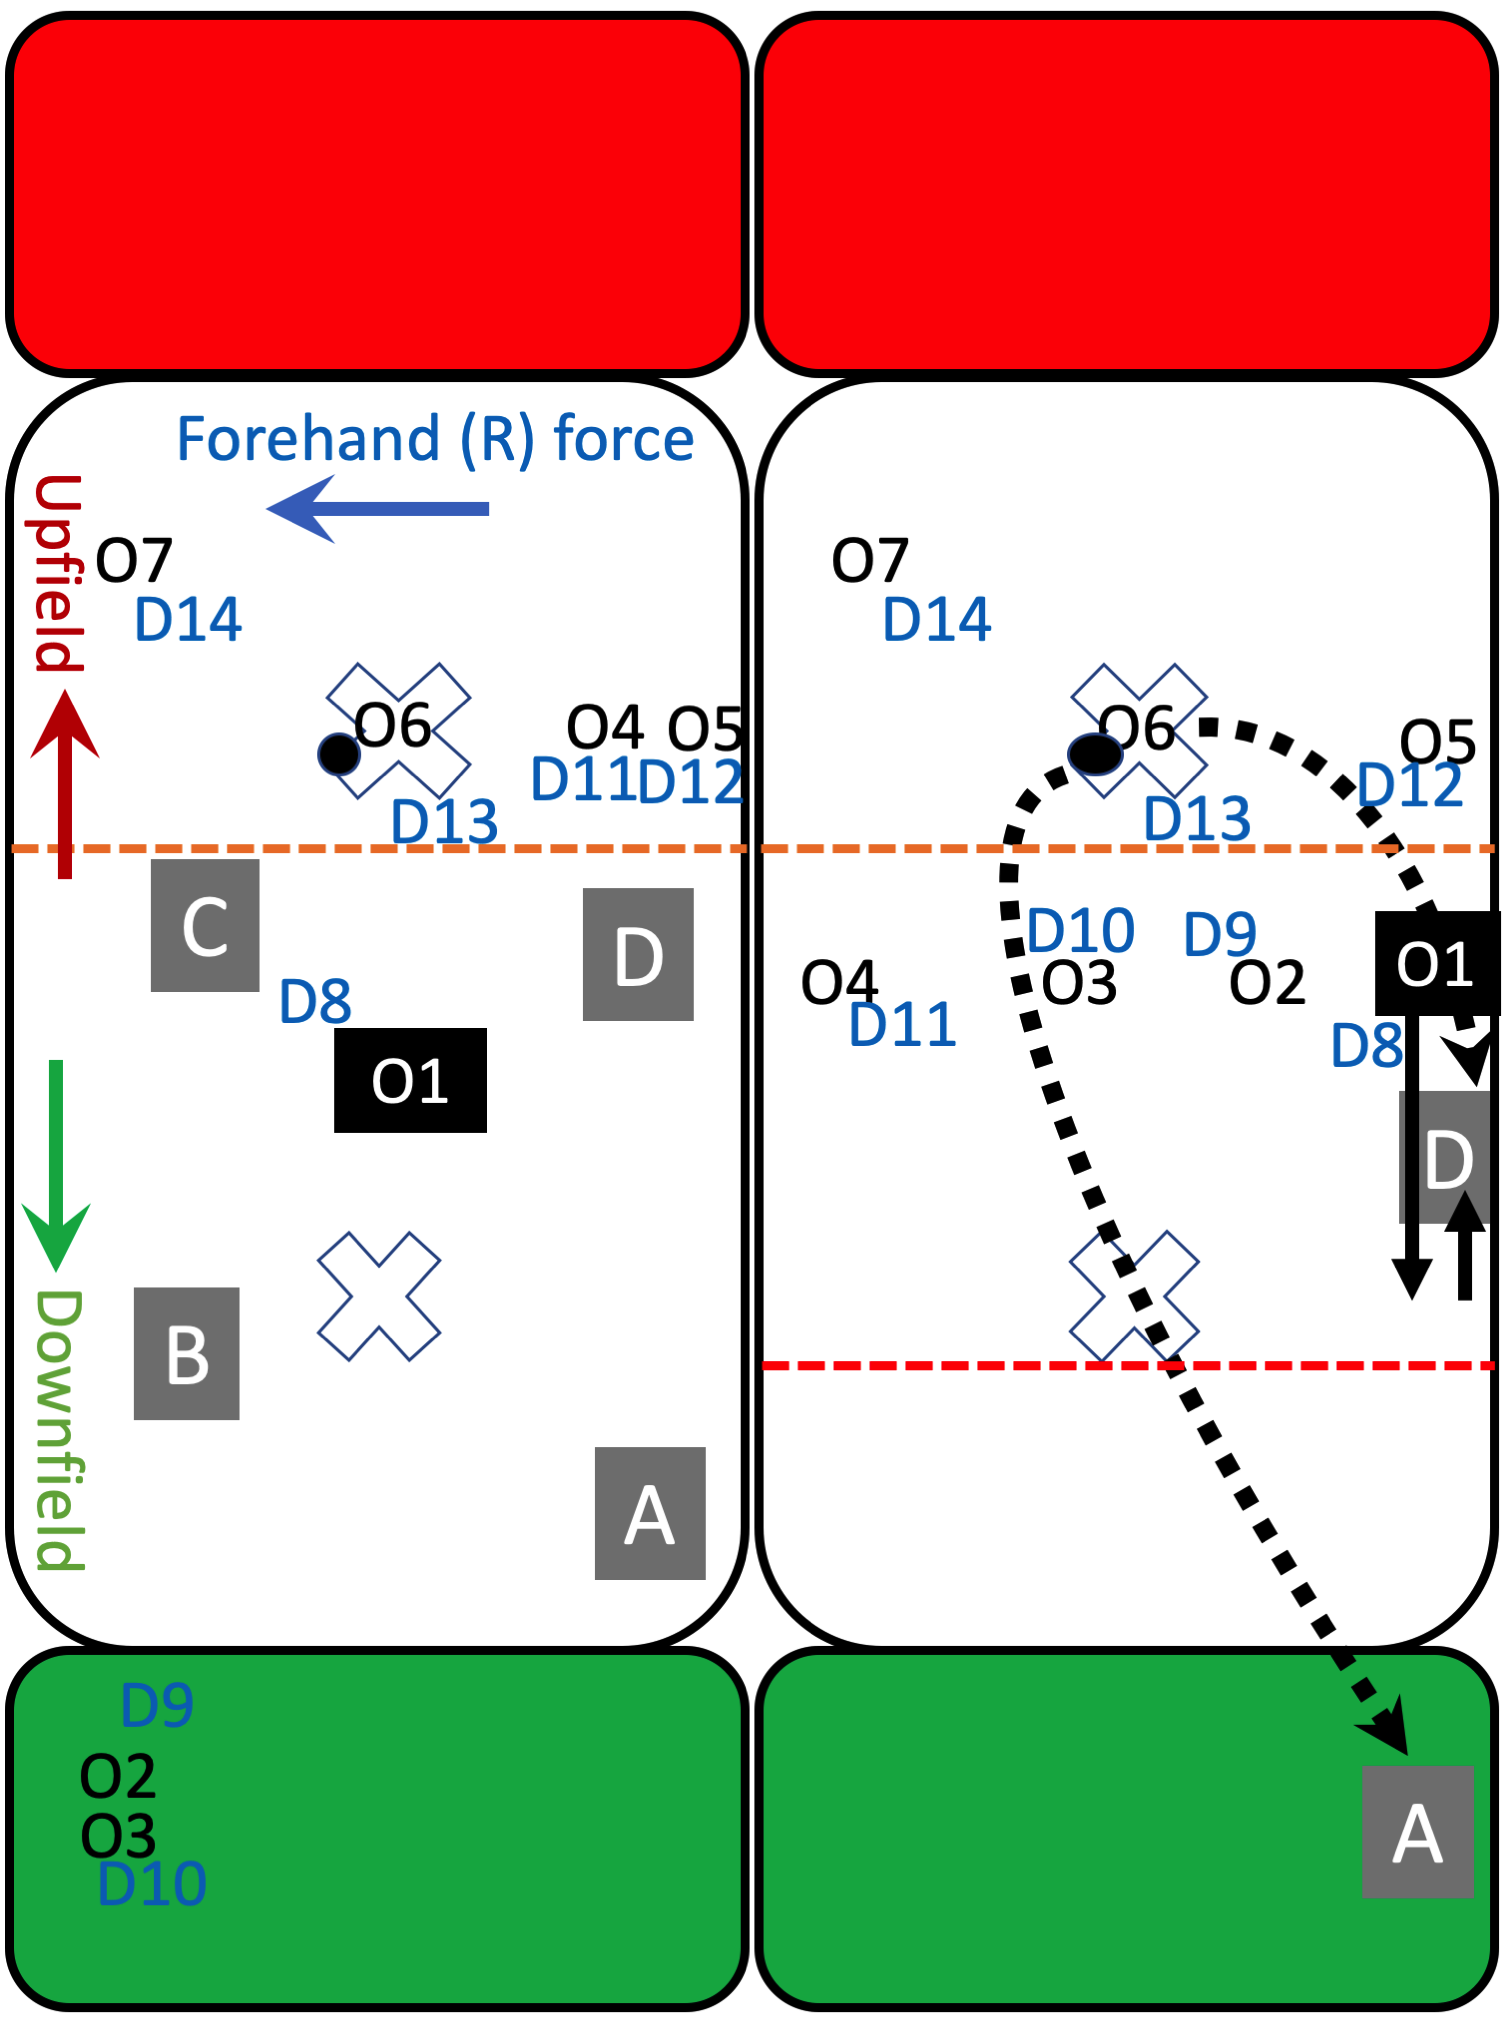
\includegraphics[width=\linewidth]{O1-horizontal}
  \caption{Horizontal stack formation}
  \label{fig:O1-horizontal}
\end{marginfigure}

\subsection{Person-match defence, forehand force: horizontal stack}\label{sec:horizontall}
Figure \ref{fig:O1-horizontal} shows 
O1 on the left wing. 
In a horizontal stack 
the strategy is to cut 
upfield and downfield (black arrows)
within your quarter of the field\footnote{
Switches to 
another quarter of the field 
can work 
(as in a diamond cut)
but usually rely on the 
other person 
(e.g. O2) 
also switching quarters 
to replace you 
on the left wing.}. 
O6 can potentially throw 
a deep huck to you downfield (A)
or a break-force throw to you (D)\footnote{
This is typically easier 
on a back-under cut, 
as shown by the black arrows,
as then there is more space 
clear of D12.}.

Once you have the disc 
it is probably best 
to move it 
back to the middle of the field 
via a dump to O5 or O6. 
However, a huck to 
A for O2 or 
to B for O4 
may be effective 
if thrown as 
a (RH) outside-in backhand or
inside-out forehand 
(to the break-side of your receivers)

In the event that 
O2, O3 or O4 
get the disc
instead, perhaps
move downfield,
to offer a deep 
or back-under cut. 

\section{Zone offence}\label{sec:zone}

\begin{marginfigure}%
  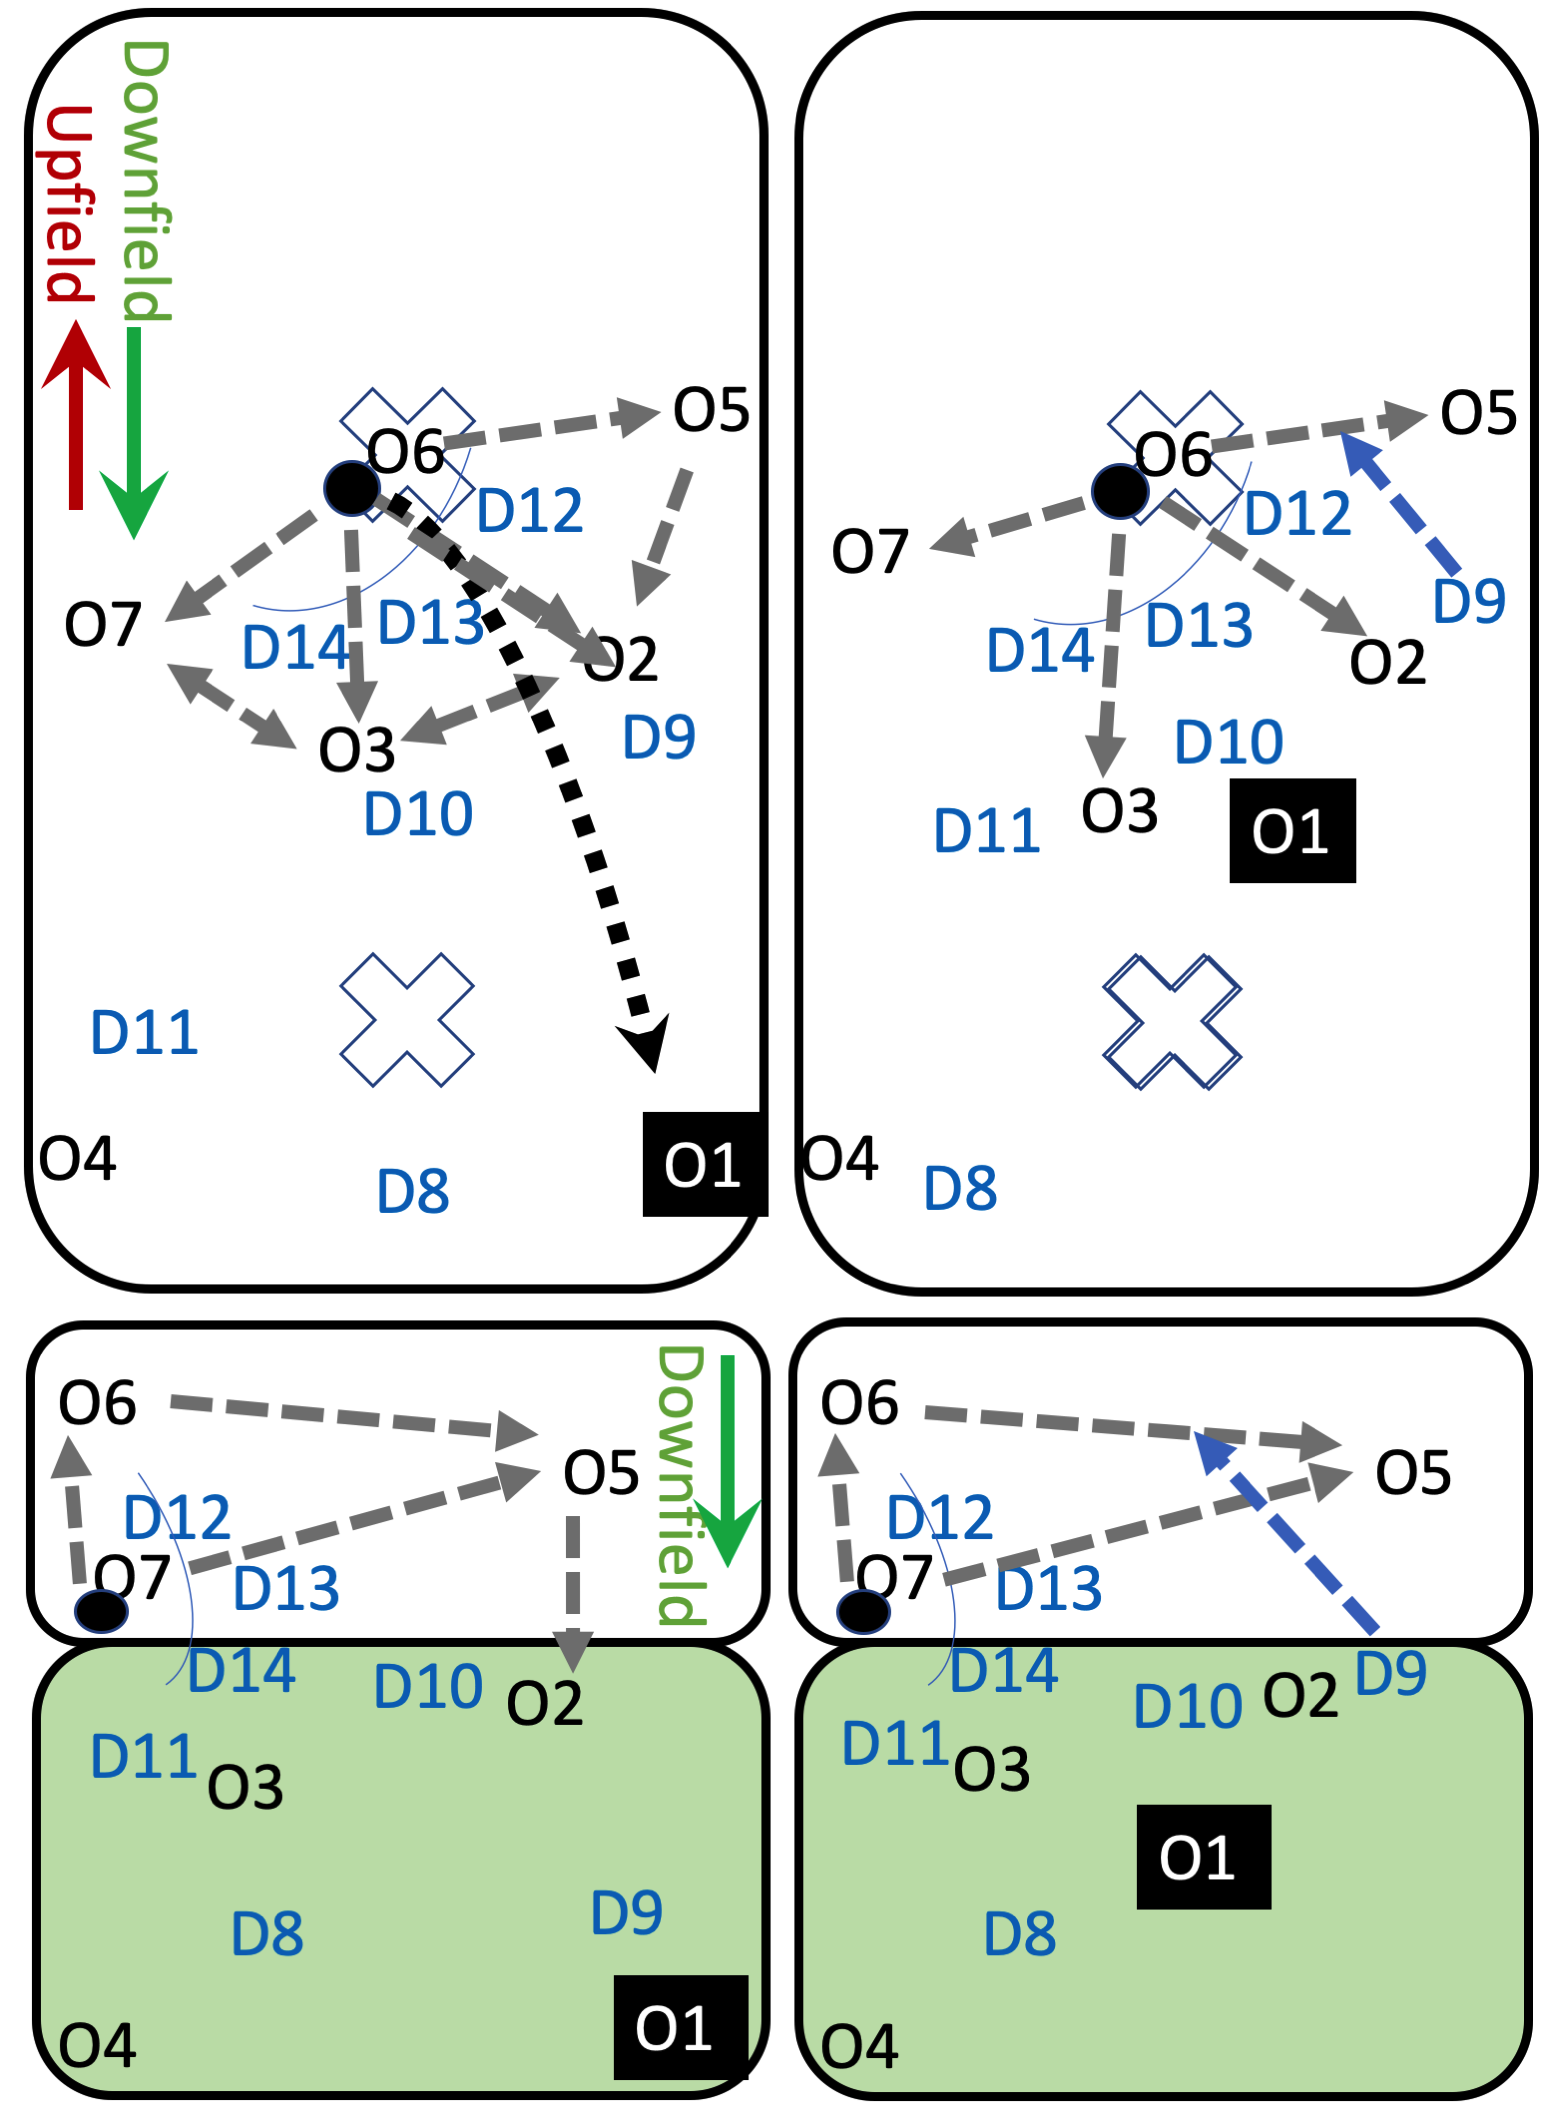
\includegraphics[width=\linewidth]{O1-zone331}
  \caption{331 zone formation}
  \label{fig:O1-zone331}
\end{marginfigure}

Oh no, 
the defence decided to play zone\footnote{
Figure \ref{fig:O1-zone331} shows a 3-3-1 zone.  
There are many other zones, 
but for the purposes of playing as O1
the principles are generally simlar.}! 
What to do? 
There are many different zones\footnote{
Even 3-3-1 might be force 
forehand, 
backhand,
middle, 
return,
sideline,
and probably more. 
Then there are 
a whole range of other formations
including:
puppy-fence (1-3-2-1),
four person cup (4-2-1)
two person cup (2,3,2) and
cup-o-saurus (6-1)!}
Regardless of what zone it is,
three ways to beat it are:
1) over;
2) round; or
3) through. 

As O1 
(left wing), 
you are mostly relevant to 
beating a zone through
(1)
\smallcaps{over}.  
This is done by exploiting the gaps between 
D8\footnote{
who is trying to cover throws 
to you or O4} 
and D9\footnote{ 
who is trying to cover you 
and O2 and 
(maybe) O5.}.
Figure \ref{fig:O1-zone331} shows 
with dashed black arrows
two potential throws from O6 to you:
\begin{enumerate}
\item O6 might throw directly to you 
(O1) where you are shown 
standing in Figure \ref{fig:O1-zone331}. 
Such a throw might be a hammer
or a blade,
because O6 will be trying to get the disc to you 
as quickly as possible, 
before either D8 or D9 can intercept it. 
Hence, it will help if you are looking directly at O6 
and standing still, 
so that they can land said throw on your head!
\item Alternatively, O6 might throw to A, 
expecting that you and the disc can get there 
before D8 does.
\end{enumerate}

The grey dashed arrows in Figure \ref{fig:O1-zone331} 
show various ways that the disc might 
go 
1) over,
2) around or
3) through 
to O5, O2 or O3. 
From them you
might receive the next pass
or the one after that
as you, collectively, 
take advantage of the 
4 (O1, O2, O3 and O5) 
versus 2 (D9 and D10)
mismatch until the 
upfield end of the zone 
(D12, D13, D14) 
catch up to the disc. 
Once they do so, 
it becomes 4 versus 5, 
so, 
as a team,
 you will likely be 
better off giving it back to 
one of the handlers 
(O5-7) 
so as to play 
7 vs 7 again. 
There are plenty of other variations,
for example, maybe it 
goes \smallcaps{(2) around}
to O7 and then deep,
taking advantage 
of the temporary 
2 (O1, O4) vs 1 (D8), 
who might have to choose 
between covering A
or B.  Regardless, 
the objective for you
as O1
is to set up 
or 2 (O1, O4) 
vs 1 (D8) 
or even 3 (O1, O4, O7) 
vs 2 (D8, D11). 
This enables your offence 
to split a defender, 
but requires that all of you
be in positions 
that can be thrown to, 
one way or another. 
Even getting a 
2 (O1, O4) 
vs 2 (D8 and D9 or D11)
downfield can be helpful, 
as then the game 
becomes 5 vs 5, 
which is easier for the offence. 


\begin{marginfigure}%
  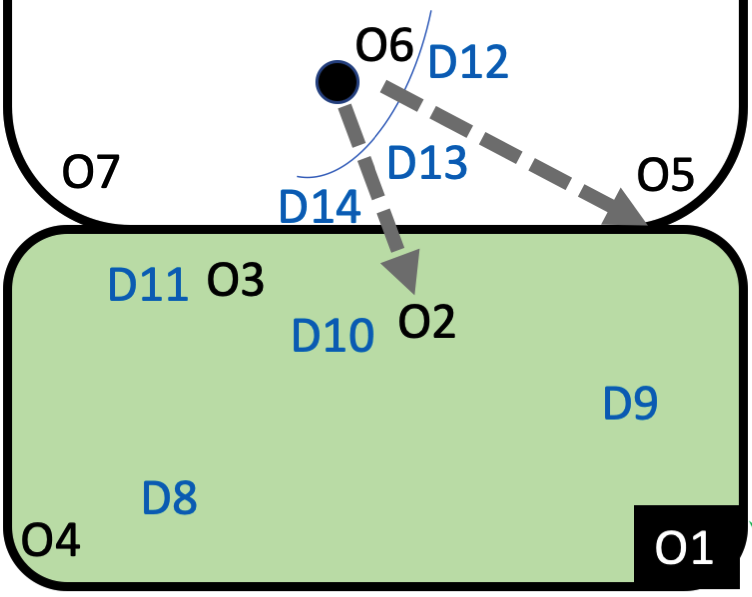
\includegraphics[width=\linewidth]{O1-zone331endzone}
  \caption{331 zone formation near the endzone}
  \label{fig:O1-zone331endzone}
\end{marginfigure}

In fact,
this should be the strategy 
if the defence 
continues to play zone 
once the disc 
gets close to the endzone, 
as shown in Figure \ref{fig:O1-zone331endzone}.
If you (O1) 
and the other wing (O4) 
go and stand 
on the back corners 
of the endzone, 
then two defenders will 
have to cover you, 
otherwise a throw \smallcaps{over}
will score\footnote{
In Figure \ref{fig:O1-zone331endzone}
D8 is shown covering O4 
(but also trying to help in the centre of the endzone)
while D9 is trying to cover O1 and O5,
and help D10 with O2.}.

\begin{marginfigure}%
  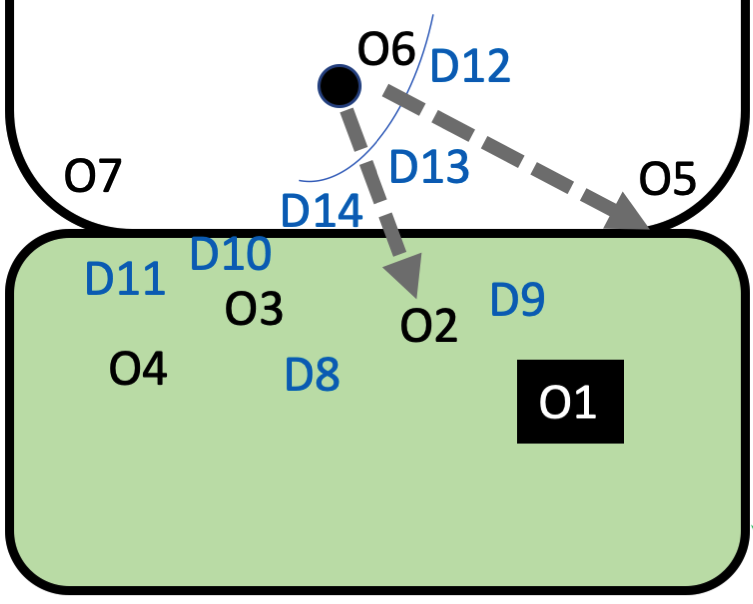
\includegraphics[width=\linewidth]{O1-zone331endzone2}
  \caption{Compressed 331 zone formation near the endzone}
  \label{fig:O1-zone331endzone2}
\end{marginfigure}

An advantage of you and O4 
being at the downfield 
corners 
of the endzone 
is illustrated through 
comparison to Figure \ref{fig:O1-zone331endzone2}.
Here O1 and O4
are further upfield
and away from the sidelines. 
This allows D8, D9, and D10 
to move upfield 
and help defend 
the front of the endzone. 
It is still possible for O6
to throw \smallcaps{over} 
into the space downfield of O1
or O4, 
however, 
this is a much harder throw. 
In Figure \ref{fig:O1-zone331endzone} 
the throw to O1 or O4 can be 
flat,
quick\footnote{
Likely, the quicker the disc gets to O1 or O4
the better,
as less time in the air 
equals less time for D8 or D9 
to get close enough to make an intercept.}
and as hard as O6 wants. 
In contrast,
the throw needed in 
Figure \ref{fig:O1-zone331endzone2} 
to pass to O1 or O4 
has to go over their (your!) head,
but be floaty enough
that it can be caught 
within the endzone. 
This appears much harder to 
throw \smallcaps{and} catch!

\section{Junk defence}\label{sec:zone}
%TALK ABOUT HOW IT'S ALL VARIATIONS ON THE THEME. FORCE THEM TO PLAY PERSON-MATCH. OR CREATE A VIABLE 2 vs 1 SITUATION.
In between zone 
and person match 
are a range of  
defensive strategies 
that are a bit of both.
The simplest is 
perhaps 
'last person back'\footnote{
In which the person who is deepest 
(furthest downfield)
switches to cover the 
offensive cutter 
who is furthest downfield 
(or the largest threat
 to receive a huck). 
The formation 
shown in Figure \ref{fig:O1-vertical} 
might involve D8 
being the 'last person back'
and so initially covering O1.  
However, once O1 
turns upfield 
D9 would switch to O1, 
with D8 subsequently covering
O2.}. 
The most complex, 
perhaps, is
'clam'\footnote{
Often called in a similar manner 
to 3-3-1 zone, 
yet with defenders effectively playing 
`person-match-with-all-the-switches'.}\footnote{
Although there's probably many 
more complex 
defensive strategies 
that I've never heard of!}.

Regardless, 
a similar approach 
to that used against zone
would seem most relevant 
to what you might do as O1. 
1) Try to spread out 
so that one defender 
cannot cover more than 
one offensive player 
(so play left wing 
and stand deep 
and wide);
2) Work with others 
on your team to try 
and find situations where 
one defender 
has to choose 
which of 2+ offensive 
players they are going to cover 
because you are arranged
such that they can't cover you all
at once!
 
That's enough for this basic document though.  
Good luck O1! 
Hopefully, 
I'll write 
more in depth 
about  zone, 
clam etc. 
in some future document. 


\end{document}
